\Chapter{Minták generálása}

\section{Tanító mintapontok előállítása}

A megvalósító neurális hálózat betanítása felügyelt tanulás módszerrel történik. A minták alapján történő tanulás lényege, hogy az eljárás során a be- és kimeneti mintapárokból igyekszünk megfelelő ismereteket kinyerni és ezzel a rendszer viselkedését módosítani. A hálózat feladata, hogy megtanulja a rendelkezésre álló mintapont párok által reprezentált bemenet-kimenet leképezést. Ehhez elő kell állítani a megfelelő adathalmazt.

Az adathalmaz előállítása elött definiálni kell a rajzolás dinamikáját. A vonal kirajzolás sorrendje mellet fontos a vonal vastagsága is. Az kézírás ugyan sokat változott, de az alapjai megmaradtak. A stroke-ok vastagsága az ecset gyorsaságától, az ecsetre ható nyomás nagyságától függ. A megfelelően rajzolt vonalakat nagyon fontosnak tartják a kínaiak, mivel a kultúrájukhoz tartozik. A kalligráfia elárulhatja az ember nemét, korát, személyességét. Kézzel írott karakterekre láthatunk néhány példát \aref{fig:calligraphy}. ábrán.

\begin{figure}[h]
\centering
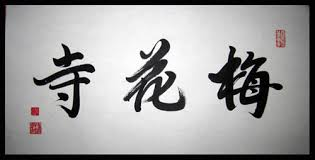
\includegraphics[scale=0.8]{images/calligraphy}
\caption{Példa néhány kézzel írott kínai karakterre}
\label{fig:calligraphy}
\end{figure}

\subsection{Vonal vastagság}

A következőkben részletezném a vonal vastagság változását a stroke-ok rajzolásának függvényében \cite{StrokeCJ9}. 

\begin{itemize}
\item A stroke-ok vége elvékonyul, ezt a valóságban az ecset hirtelen felemelésével érik el. (Van néhány kivétel, mint például a \textit{right fally} 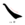
\includegraphics[scale=1.0]{right_fally}) 
\item Ha egy stroke végéből kezdődik egy másik stroke, akkor azok találkozásánál a vonalvastagság növekszik.
\item A horizontális vonalak közepe elvékonyul majd a végén újra vastagabb lesz (\ref{fig:vastagsag}. ábra). A vastagságot súlyokkal könnyedén lehet definiálni.

\begin{figure}
\centering
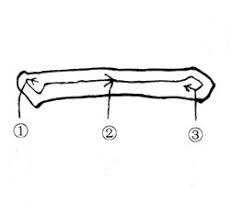
\includegraphics[scale=0.6]{images/horizontal_line}
\caption{Vonal vastagságának változata a vonások egyes részeinél}
\label{fig:vastagsag}
\end{figure}

\item A kampós vonalaknál (hooked stroke) a "kampó" hirtelen vékonyodással és irányváltoztatással jár. Az ecset hirtelen felemelésével érik el. Általában a kampó 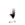
\includegraphics[scale=1.0]{hook} stroke része.
\item A további stroke-ok általában állandó vonal vastagsággal (ecset gyorsaság állandó). A kézzel írás és festés egyén függő.
\end{itemize}

\subsection{Környezet a karakterek kirajzolásához}

\begin{itemize}
\item A kínai karakterek festése papíron történik. A mi esetünkben ez a képernyő. A karakterek fekete-fehér színüek. A szürke árnyalatokat $[0, 255]$ intervallumon vett egész értékek reprezentálják. Az ideálisan kirajzolt karakter fekete-fehér színű, és ahhoz a generálás során adhatunk hozzá szürke pixelek formájában zajt.

A karakterek rajzolásához a Python programozási nyelv és a hozzá elérhető eszközök használata tünt megfelelő választásnak. Egy $512 \times 512$ pixelből álló fehér kép kirajzolása az alábbi módon történik a segítségével.
\begin{python}
img = np.zeros((512, 512, 3), np.uint8)
img[0:512] = (255, 255, 255)
\end{python}

\item A festés alapvető eszköze az ecset. Az ecset lenyomássa egy ellipszis alakot hozz létre. A festés során az ecset elfordul (megfigyelésünk szerint 45fokban). Az ellipszis területe megnő, ha a festés gyorsasága csökken, ellenkező esetben csökken. Az ellipszist könnyedén lehet rajzolni az OpenCV \texttt{ellipse} függvénye segítségével, amelynek a paraméterezése a következő.
\begin{python}
cv2.ellipse(img, center, axes, angle, start_angle, 
	end_angle, color, thickness=1, lineType=8, shift=0) 
\end{python}
\end{itemize}

\subsection{Karakterek kirajzolása}

A kínai karaktereket különféle módokon reprezentálhatjuk. Ezek közül néhány lehetőséget mutatnak be az alábbi pontok.

\begin{enumerate}
\item \textit{Poligonos közelítés}: A kínai karakter kontúrját ebben az esetben, mint poligont adhatjuk meg. Minél több éllel definiáljuk a karaktert, annál jobb minőségű képet érünk el, viszont a számítás igényünk növekszik.
\item \textit{Procedurális rajzolás}: Ebben az esetben a karakter kirajzolásának a procedúráját adhatjuk meg. Amennyiben feltételezzük, hogy az ecsetünk ellipszis alakú, úgy kitöltött ellipsziseket egymás után, kis lépésközzel kirajzolva. Az ellipszisek pozíciója mellett azok méretét is változtathatjuk. A közelítési módra egy példát láthatjuk \aref{fig:proc_draw}. ábrán.

\begin{figure}
\centering
\begin{tabular}{ c c }
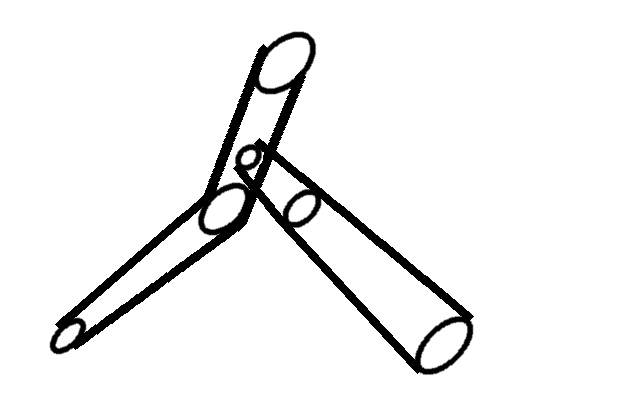
\includegraphics[scale=0.25]{images/proc_draw1} & 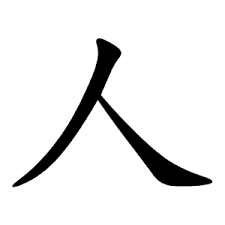
\includegraphics[scale=0.5]{images/ren}
\end{tabular}
\caption{Karakter közelítése változó méretű ellipszisekkel}
\label{fig:proc_draw}
\end{figure}

Az ellipszisek koordinátáit egy-egy 5 dimenziós vektorral adhatjuk meg
\begin{align*}
P_1 &= (x_1, y_1, d_{x_1}, d_{y_1}, s_1) \\
P_2 &= (x_2, y_2, d_{x_2}, d_{y_2}, s_2).
\end{align*}
Az $x$ és $y$ koordináta párral az ellipszis középpontját adjuk meg. A $d_x$ és $d_y$ a kirajzolandó görbe végpontjaiban vett érintő irányvektora. Az $s$ az ellipszis méretét adja meg. Meghatározza, hogy mennyire gyors az ecsetvonás, a kirajzolt ellipszis területével arányos. Az ecset dinamikája olyan, hogy lassú ecsetmozgás nagyobb, vastagabb vonalakat eredményez, míg a gyors általában véknyabbakat. Az íveken mozgatott változó méretű ellipszisek használatát szemlélteti \aref{fig:proc_draw2}. ábra.

\begin{figure}
\centering
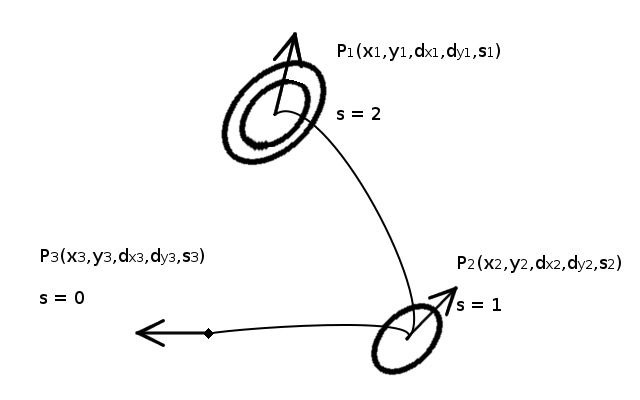
\includegraphics[scale=0.5]{images/proc_draw2}
\caption{A karakterek összeállítása íveken mozgatott ellipszisek segítségével}
\label{fig:proc_draw2}
\end{figure}

A görbék kirajzolásához egy megfelelő megoldást ad a Hermit ívek alkalmazása. Ezek olyan harmadfokú görbék, melyeknek a két végpontja, és a végpontokban vett érintők rögzítettek.

Jelölje $\textbf{H}$ a Hermit ívünket, amelynek $u \in [0, 1]$ a paramétere. Ezt a
$$
\textbf{H}(u) = \textbf{a}_0 u^3 + \textbf{a}_1 u^2 + \textbf{a}_2 u + \textbf{a}_3
$$
alakban írhatjuk föl, ahol az $\textbf{a}_i$ értékek a görbe helyére és alakjára vonatkozó konstansok. Tekintsünk egy $\textbf{p}_0$ és $\textbf{p}_1$ pontot, illetve a hozzájuk tartozó $\textbf{t}_0$ és $\textbf{t}_1$ érintőket. A vonások leírásához használt paraméterek alapján ezek az alábbiak lesznek:
$$
\textbf{p}_0 = [x_1, y_1], \quad
\textbf{p}_1 = [x_2, y_2], \quad
\textbf{t}_0 = [d_{x_1}, d_{y_1}], \quad
\textbf{t}_1 = [d_{x_2}, d_{y_2}].
$$

A Hermit ív együtthatóit a következő képpen tudjuk kiszámítani:
\begin{align*}
\textbf{a}_0 &= -2(\textbf{p}_1 - \textbf{p}_0) + \textbf{t}_0 + \textbf{t}_1, \\
\textbf{a}_1 &= 3(\textbf{p}_1 - \textbf{p}_0) - 2 \textbf{t}_0 - \textbf{t}_1, \\
\textbf{a}_2 &= \textbf{t}_0, \\
\textbf{a}_3 &= \textbf{p}_0.
\end{align*}

Tekintsük azt az esetet, amikor a görbén köröket mozgatunk. Ennek a számításához vezessük be a $\textbf{b}_i$ értékeket, amelyet a
$$
\textbf{b}_i = [-y, x] \quad \Leftrightarrow \quad \textbf{a}_i = [x, y]
$$
formában adhatunk meg. Ennek segítségével a görbe adott pontjához tartozó egység hosszúságú normálvektort az
$$
\textbf{n}(u) = \dfrac{3 \textbf{b}_0 u^2 + 2 \textbf{b}_1 u + \textbf{b}_2}{
||3 \textbf{b}_0 u^2 + 2 \textbf{b}_1 u + \textbf{b}_2||
}
$$
alakban kapjuk.

A görbe egyes pontjaihoz tartozó kör méretét az alábbi módon számíthatjuk ki az $u$ függvényében:
$$
s(u) = (1 - u) \cdot s_1 + u \cdot s_2.
$$

A vonáshoz tartozó két (\textit{hosszanti}) kontúr görbét ezekből a
$$
\textbf{z}(u) = \textbf{H}(u) \pm s(u) \cdot \textbf{n}(u)
$$
alakban írhatjuk föl. Ez tehát tulajdonképpen két görbét ír le, amelyek a normálvektorok számításánál lévő hosszmeghatározás miatt nem írhatók föl Hermit ívként.

A körökből ellipsziseket utólagos transformációval is kaphatunk, vagyis ha a kapott közelítő sokszög pontjait utólag a görbe mentén adott irányba arányosan eltoljuk.

\item \textit{Pontonkénti színszámítás}: A képernyőn megjelenített képet lehet úgy tekinteni, mint egy $n \times m$ méretű mátix (képernyő szélessége: $m$, magassága: $n$). Az egyes pixelek értékét az algoritmussal külön-külön is meghatározhatjuk.

\end{enumerate}

A három karakter kirajzolás közül a procedurális rajzolás a leginkább hatékony.

\subsection{Karakter zajosítás}

A zajok hozzáadását OpenCV-ben könnyedén meg lehet valósítani \cite{OpenCVli86}. Különféle zajosítási módokat szoktak használni \cite{WANG1973303}, amelyek közül a jelentősebbeket az alábbi pontok mutatják be.

\begin{itemize}
\item Pontszerű zajok

Tételezzük fel hogy a karakterünk mátrixa $M$ és zaj mátrixunk $N$ van. A két mátrix sor és oszlop száma megegyezik.
$$
M = \left(
\begin{array}{ccccccc}
1 & 1 & 1 & 1 & 1 & 1 & 1 \\
0 & 1 & 0 & 1 & 0 & 1 & 0 \\
1 & 0 & 0 & 1 & 1 & 0 & 0 \\
0 & 0 & 1 & 1 & 0 & 0 & 1 \\
1 & 1 & 1 & 0 & 0 & 0 & 0 \\
0 & 1 & 0 & 0 & 1 & 0 & 1 \\
1 & 0 & 0 & 0 & 0 & 1 & 1 \\
0 & 0 & 1 & 0 & 1 & 1 & 0 \\
\end{array}
\right),
\quad
N = \left(
\begin{array}{ccccccc}
0 & 0 & 0 & 0 & 0 & 0 & 0 \\
1 & 0 & 1 & 0 & 1 & 0 & 1 \\
0 & 1 & 1 & 0 & 0 & 1 & 1 \\
1 & 1 & 0 & 0 & 1 & 1 & 0 \\
0 & 0 & 0 & 1 & 1 & 1 & 1 \\
1 & 0 & 1 & 1 & 0 & 1 & 0 \\
0 & 1 & 1 & 1 & 1 & 0 & 0 \\
1 & 1 & 0 & 1 & 0 & 0 & 1 \\
\end{array}
\right).
$$

M $\oplus$ N (a bináris operátor $\oplus$ később kerül meghatározásra). Fizikailag a zaj helytelen nyomtatási folyamatot jelent, vagy olyan helyzetet, amikor a felismerési rendszerben lévő gépi zaj torzítja a mintát. Feltételezzük továbbá, hogy minden egyes cellához tartozik zaj.
Ha egy adott cella $(i, j)$ zajszintje nagyobb, mint az 1 vagy "fekete", akkor 1-re kvantálódik. Más szavakkal, minden cella végül 1 vagy 1 besorolásnak kell alávetni. Megállapíthatjuk tehát, hogy a fent említett bináris művelet a következőket jelenti: 0 $\oplus$ 0 = 0, 0 $\oplus$ 1 = 1, 1 ~ 0 = 1, és 1 $\oplus$ 1 = 1.
A zaj mátrix elemeinek megválasztásával különböző pontszerű zajokat tudunk létrehozni.

\item Elmosódások

Az elmosódás, amit símitásnak is neveznek, egyszerű és gyakran használt képfeldolgozási művelet. A simításnak sok oka van. A zaj növelése érdekében a elmosódás összpontosítunk.

Az elmosódás művelet végrehajtásához szűrőt alkalmazunk a képünkre. A szűrők legáltalánosabb típusa lineáris, amelyben a bemeneti pixelértékek (azaz $f(i+k, j+l)$) súlyozott összegével határozzák meg a kimeneti pixel értékét. Jelölje a pixel értékét $g(i, j)$. Ekkor ezt a
$$
g(i, j) = \sum_{k, l} f(i + k, j + l) h(k, l)
$$
formában számolhatjuk, ahol $h(k, l)$-t a kernelnek nevezik, ami nem más, mint a szűrő együtthatói.

Sokféle további szűrő létezik, mint például: Normalizált szűrő, gauss szűrő, medián szűrő.

A normalizált szűrő a legegyszerűbb. Minden kimeneti pixel a kernel szomszédainak átlaga (mindegyik egyenlő súlyokkal jár)

A kernel az alábbi:

\[K = \dfrac{1}{K_{szélesség} \cdot K_{magasság}} \;
\cdot
\left[
\begin{matrix}
    1 & 1 & 1 & ... & 1 \\
    1 & 1 & 1 & ... & 1 \\
    . &. &. & ... & 1 \\
    . &. &. & ... & 1 \\
    1 & 1 & 1 & ... & 1   
\end{matrix}
\right].
\]
\item Forgatás

Egy kép elforgatását $\theta$ szöggel az alábbi mátrix formájában írhatjuk föl:
$$
M = \begin{bmatrix} cos\theta & -sin\theta \\ sin\theta & cos\theta   \end{bmatrix}.
$$
Az OpenCV azonban skálázható elforgatással rendelkezik, állítható forgó centrummal, így tetszőleges helyre forgatható. A módosított transzformációs mátrixot a

$$\begin{bmatrix}
\alpha &  \beta & (1- \alpha )  \cdot center.x -  \beta \cdot center.y \\ - \beta &  \alpha &  \beta \cdot center.x + (1- \alpha )  \cdot center.y
\end{bmatrix}$$

ahol:

$$\begin{array}{l}
\alpha =  scale \cdot \cos \theta , \\ \beta =  scale \cdot \sin \theta
\end{array}$$

Ennek az átalakulási mátrixnak a megtalálásához az OpenCV egy \\ \texttt{getRotationMatrix2D} függvényt biztosít.

\begin{python}
img = cv2.imread('chinese_char1.png', 0)
rows,cols = img.shape

M = cv2.getRotationMatrix2D((cols/2, rows/2), 90, 1)
dst = cv2.warpAffine(img, M, (cols, rows))
\end{python}

\item Vágás

A grafikában a kivágás: a nem kívánt területek eltávolítása egy képből. Az egyik legegyszerűbb fotó manipulációs folyamat, ami eltávolítja a nem kívánt stroke részletet vagy releváns pixeleket a karakteren. A képarány változatlan marad, az összetétele változik. A képsíkon akár függvénnyel is megadható, hogy mely részeket távolítsuk el.

\begin{python}
import cv2
img = cv2.imread("chinese_char1.png")
crop_img = img[y:y+h, x:x+w]
cv2.imshow("cropped", crop_img)
cv2.waitKey(0)
\end{python}

\item Takarás

A takarási feladat megoldásának több lehetséges módja van, mint például: festő algoritmus, z-buffer, Warnock algoritmus, láthatósági gráfok.

A festő algoritmus egszerű és párhuzamosítható. Ennek az algoritmusnak az alapgondolata, hogy a megjelenítendő objektumokat a nézőponttól való távolság függvényében sorba kell állítani. Az algoritmus a helyes takarási viszonyokat úgy alakítja ki, hogy a nézőhöz közelebb eső objektum képe felülírja a távolabbi objektum képét. Ennek legegyszerűbb változata az úgynevezett festő algoritmus, mely a képfestés technikájához hasonlóan a távolabbi objektumokra ráfesti a közelebbieket.
Lépések:
\begin{itemize}
\item Rendezzük a poligonokat a legkisebb (legtávolabbi pontjaik) z koordinátáik szerint.
\item Hátulról előre haladva fessük ki a poligonokat. 
\end{itemize}

\end{itemize}